\begin{figure*}[!ht]
\centering
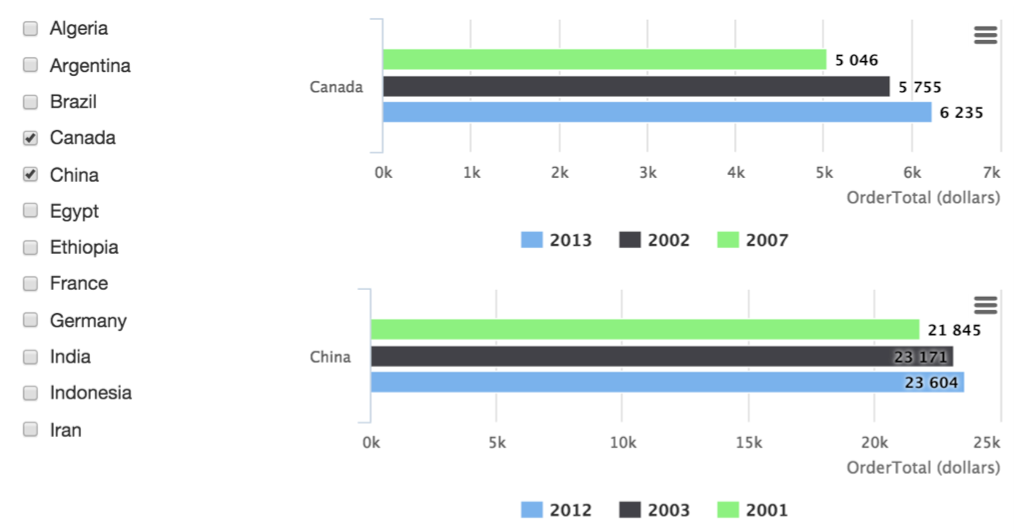
\includegraphics[width=14cm]{images/complex-example}
\caption{Monitor Top 3 Years of amount spent for selected countries (Example 2)}
\label{fig:complex-example}
\end{figure*}

\begin{figure*}[p]
\centering
\begin{minipage}{0.45\textwidth}
\centering
\begin{Java}[basicstyle=\small]
public List getSumTotal3Years(List selectedNations)  {
  List sumTotals = new ArrayList();
  PreparedStatement stmt = conn.prepareStatement(
      "SELECT order_year, sum(o.total_price) as sumTotal\n"
   + "FROM Orders o, Customers c\n"
   + "WHERE o.cust_ref = c.cust_key\n"
   + "AND c.nation_ref = ?\n"
   + "GROUP BY o.order_year\n"
   + "ORDER BY sumTotal DESC\n"
   + "LIMIT 3");
   for (Nation nation : selectedNations) {
      stmt.setInt(1, nation.getNationKey());
      ResultSet rs = stmt.executeQuery();
      List pairs = new ArrayList();
      while (rs.next()) {
         int year = rs.getInt("order_year");
         int total = rs.getInt("sumTotal");
         pairs.add(Pair.of(year,total));
      }
      sumTotals.add(pairs);
   }
   return sumTotals;
}
\end{Java}
\caption{Java Code for Example 2}
\label{fig:code-complex}
\end{minipage} \hfill
\begin{minipage}{0.45\textwidth}
\centering
\begin{SQL}
SELECT n.nation_key, n.name, (
  SELECT order_year,
         sum(total_price) as sum_price
  FROM db.orders AS o,
       db.customers AS c
  WHERE o.cust_ref = c.cust_key
  AND c.nation_ref = n.nation_key
  GROUP BY order_year
  ORDER BY sum_price DESC
  LIMIT 3
) AS aggregates
FROM session.selected_nations AS s,
     db.nations AS n
WHERE s.nation_ref = n.nation_key
AND  s.selected = true
\end{SQL}
\caption{SQL++ Code For Example 2}
\label{fig:complex-query}
\end{minipage} \hfill
\centering
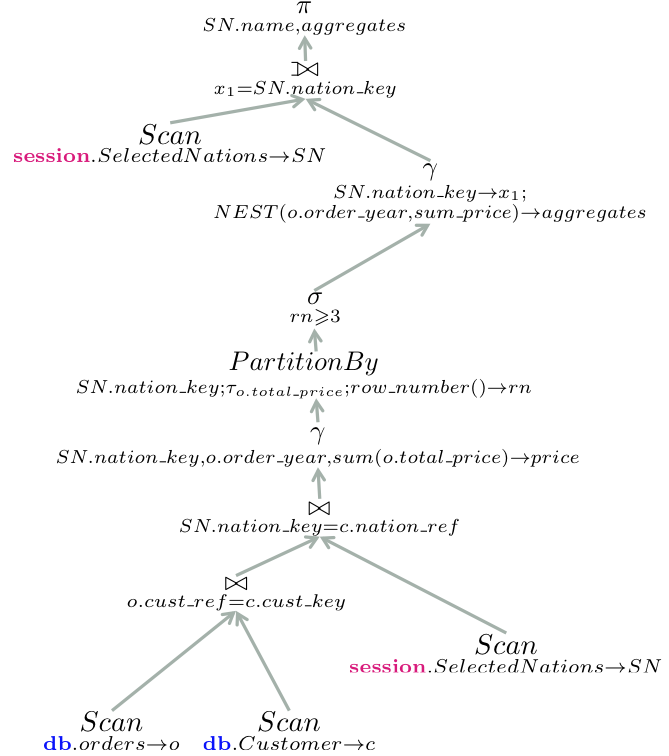
\includegraphics[width=8cm]{images/distributed-complex-plan}
\caption{Set-at-a-time rewritten plan for example 2}
\label{fig:complex-example-plan}
\end{figure*}

Consider the extension to the running example shown on figure \ref{fig:complex-example}, in which the top three years of sales revenue are displayed instead of the total revenue across all years. The Java code for this extension using the parameter-at-a-time technique is shown on figure \ref{fig:code-complex}.

The query shown (on lines 4-10), computes the top three years in terms of sales revenue for a parameterized nation. The lines 15 to 18 collects the year and sum into a list called \texttt{pairs} before adding them to the output list. In this situation, for each parameterized query, a \emph{list} of values is obtained from the database instead of a scalar. In this situation, the batched form of the complex  would violate the first normal form, and cannot be expressed using SQL. In this context, the query batching and query synthesis approaches, which are based on the relational data model, can't be used. 

SQL++, however, can operate over semi-structured data. Figure \ref{fig:complex-query} shows a SQL++ query for example 2. Lines 2-10 display a \emph{correlated subquery} which returns the 3 top years for the nation bound to variable $n$.

The FORWARD query processor represents a correlated subquery using the \emph{ApplyPlan} operator, which takes as input a semi-structured record $t = \{a_1:v_1, ..., a_n:v_n\}$ and a plan $p$. It evaluates plan $p$ over $t$ to value $w$, and outputs a new record $\{a_1:v_1, ..., a_n:v_n, b:w\}$. Note that values $v_1, ..., v_n, w$ may be themselves scalars, records, or even list of records. Note that variables $a_1,...,a_n$ of the input binding tuples appear as parameters in $p$ wherever constants or variables can appear in uncorrelated plans. The \emph{GroupBy} operator (also denoted $\gamma$) can also generate nesting, through the \emph{Nest()} aggregate function, which instead of outputting a scalar outputs the list of records with the same grouping values. 

In our running example, the FORWARD query processor parses the query on figure \ref{fig:complex-query} and produces an initial logical plan using the ApplyPlan operator. It then removes the apply-plan operator using a set-at-a-time rewriting rule \cite{yupeng-fu:2014aa} and produces the distributed plan shown on figure \ref{fig:complex-example-plan}. This plan has a number of differences with the relational set-at-a-time plan : 

\begin{itemize}
\item{Notice that the nesting in the rewritten plan is produced by a $\gamma$ operator with the \emph{Nest()} aggregation function. Given that the \emph{Nest()} aggregation cannot be performed by the relational database, it is performed by the FORWARD middleware.}
\item{The \emph{PartitionBy} operator applies the ordering over the partitions formed by the nation keys, which allows the sorting of the different groups within the relational database.}
\end{itemize}

Only a single denormalized query is sent from to the database in this example, while the \emph{Nest()} aggregation function is used to create the nested lists. 

\subsection{Integrated Query Languages}
%% Short Version

Another approach taken by researchers to integrate nested data into application programming languages has been through \emph{Integrated Query Languages}. One of the most popular implementations is Microsoft's LINQ \cite{LINQ},  which integrates seamlessly a declarative query facility within the application programming language. With LINQ, developers use Standard Query Operators (SQOs) to formulate queries against both application objects, database-resident data and XML files. The queries are eventually translated into SQL or XQuery if they target database data or XML data, respectively. Here is an example of a LINQ program for Example 2. On line 1, the \texttt{n} variable is bound to the table \texttt{nations} and filtered according to the \texttt{Where} SQO. The \texttt{Select} SQO is used lines 2-10 to collect the top 3 years data. This code will also produce a parameter-at-a-time execution, as LINQ will produce a separate SQL query for each invocation of the \texttt{Select} SQO. 

\begin{SQL}
var result =
	from n in db.nations
	where selectedKeys.Any(key => key == n.nation_key))
	select new {
		name = n.name,
		aggregates = (from c in db.customers
		where c.nation_ref equals n.nation_key
		join o in orders on c.cust_key == o.cust_ref
		group o by o.order_year into g
		select new {
			order_year = g.order_year,
			sum_total = g.sum(t => t.total_price)} into ag
		orderByDescending ag.sumTotal
		limit 3)
	}
\end{SQL}

Gurst \cite{gurst:2010aa} presents a way to translate the SQOs into algebraic plans through a technique called \emph{loop lifting} \cite{gurst:2004aa, gurst:2009aa}. The algebraic plans themselves can then be translated to SQL. A single LINQ query translation can have multiple plan roots, possibly with common-subexpressions. However, the number of plan roots is limited by level of nesting in the query result type. This technique guarantees that it is only a LINQ query's static result type, and not the size of the database, which determines the number of SQL queries produced. Gurst extended his work to the Ruby programming language with the SWITCH tool \cite{gurst:2013aa}. 
